%!TEX root = main.tex

\section*{Introduction}

Genetic clustering algorithms are commonly used to describe genetic structure among populations, reflecting the cumulative
effects of isolation, connectivity (i.e., genetic migration), selection, and genetic drift.  The ability of such algorithms to differentiate populations
is limited by the extent of genetic differentiation among populations and the capacity to resolve those differences given the available marker
set and sample sizes from the respective populations.  Based on an initial description of genetic structure, ecologists are frequently
interested in describing patterns of genetic movement among populations, often inferred from the mismatch between the sampling location
and genetic origins of a given individual \citep{paetkau1995microsatellite,wilson2003bayesian}.  Genetic movement has many implications,
such as influencing evolutionary processes, maintaining genetic variation through gene flow, driving disease dynamics and affecting patterns
of invasive species expansion \citep{huestis2019windborne, estoup2010reconstructing}.

In using clustering algorithms to describe genetic structure among natural populations, researchers frequently identify individuals of
mixed ancestry---individuals with proportions of their genome attributed to multiple subpopulations, sensu \citet{pritchard2000inference}.
Various processes could contribute to the appearance of mixed ancestry in a clustering analysis.  Most directly, individuals may represent the
influences of gene flow among populations, occurring in recent or prior generations, with the observed complex ancestry patterns accurately
representing contributions from multiple sampled populations.  However, similar patterns may result from functionally different patterns of
population structuring.  For example, such patterns might be expected when clinal systems governed by isolation by distance are described
as discrete genetic clusters.
Alternatively, individuals of mixed ancestry could reflect immigration from outlying populations (e.g., exogenous immigration), with true source
populations not sufficiently
represented in the sample to be among the characterized $K$ subpopulations.
Furthermore, the characterization of admixed individuals may reflect a limitation of the statistical power of the genetic data,
as a function of both the marker set and sample size, to resolve the true underlying patterns of genetic structure.
 The challenge for researchers then becomes correctly identifying the ecological and/or statistical processes by which observed complex
 ancestry patterns were created.

A best practice for evaluating the behavior of genetic clustering algorithms on an empirical dataset is to conduct
parallel analyses on data that have been simulated---so the truth is known---so as to mirror the empirical data set
as closely as possible \citep{vaha2006efficiency,anderson2008improved,latch2011fine}.
Techniques to simulate individual genotypes in this context frequently use sampling with replacement from the
observed allele frequencies (see, for example, \citealt{nielsen2006hybridlab,kinziger2008hybridization}).
However, sampling with replacement implicitly increases the pairwise genetic distance among simulated samples, relative to the observed
samples, and
inflates the perceived statistical power to correctly assign individuals back to source populations.
We refer to this phenomenon as resampling-induced, spurious power inflation (RISPI).
\citet{anderson2008improved} used simulations to document this type of artifact in the context of
genetic stock identification (GSI), a type of clustering application in which individuals are constrained to have
all their ancestry from a single subpopulation.
Similar statistical artifacts occur when simulating data to
assess how accurately admixture fractions can be estimated.


Beyond simply evaluating the resolution of discrete populations in a simulated framework, researchers may also be
interested in how individuals of admixed ancestry are genetically characterized given the statistical power of the available dataset and the
analysis methods used.
Recognizing that connectivity among genetically distinct populations may be relatively rare, additional insight into the
frequency of immigration can be gained by integrating across generations to identify both direct migrants and descendants of migrants
 (i.e., F1 hybrids or advanced hybrids reflecting the effect of backcrossing across multiple generations [BC1, \ldots,
BCX]).
Evaluating the results of genetic clustering algorithms in the context of data that are
expected to arrive by such a process of hybridization requires simulation of
explicit hybrids.  Such simulations are the purpose of the software {\sc hybridlab} 
\citep{nielsen2006hybridlab}.

%%%%%%%%%%%
\begin{figure}
\newcommand{\gspcapone}{\footnotesize
A genomic simulation pedigree (GSP) for simulating $F_2$ individuals.
Squares denote founder and non-founder nodes in the pedigree. There are four founders in the pedigree,
individuals 1--4.  The  triangles above each of those founders denotes, in color
and text, the population of origin of each of the two genomes within each founder.
Thus, individuals~1 and~2 are founders purely from population~$A$, and~3 and~4
are purely from population~$B$.  The pink hexagon labeled s7 is the sample node.
It represents samples that are taken from non-founder node~7, which, from the structure
of the pedigree, clearly represents an $F_2$ hybrid between populations $A$ and $B$.  The red numbers
on edges above and leading into each non-founder node indicate the number of
gametes that get segregated from the parent node (at the top of the edge) to the
daughter node (at the bottom of the edge).
This emphasizes that,
in dropping genes through a GSP, in contrast
to a traditional pedigree, each parent
node may segregate multiple gametes to a daughter node.  See the text for
further explanation.
Each non-founder node $x$ will have exactly two edges coming into it from above
(from its two parents), and we denote the numbers associated with those edges as $G^+_{x,1}$ and $G^+_{x,2}$.
For example, node 6 has $G^+_{6,1}=G^+_{6,2} = 2$.
A founder individual may have, at most, 2 edges coming downward out of it, while a non-founder individual may have more or less than two edges coming downward
out of it.  Letting $e_x$ be the number of downward edges out of node $x$ to its $e_x$
non-founder daughter nodes, we denote the number of gametes segregated
through each edge as $G^{-}_{x, 1},\ldots,G^{-}_{x, e_x}$.  For example, at
non-founder node~5, $e_5 = 1$ and $G^{-}_{5,1}=4$.
Finally, the purple number adjacent to the edge leading into the
sample node indicates how many sample individuals are drawn from individual
node 7. Any non-founder individual node can have a maximum of one edge leading
to a sample node.  We denote the number of samples emanating from node $x$ as $S_x$. In our example $S_7=4$ indicates that four $F_2$ individuals are
created from a single simulation on this GSP.
}
\begin{center}
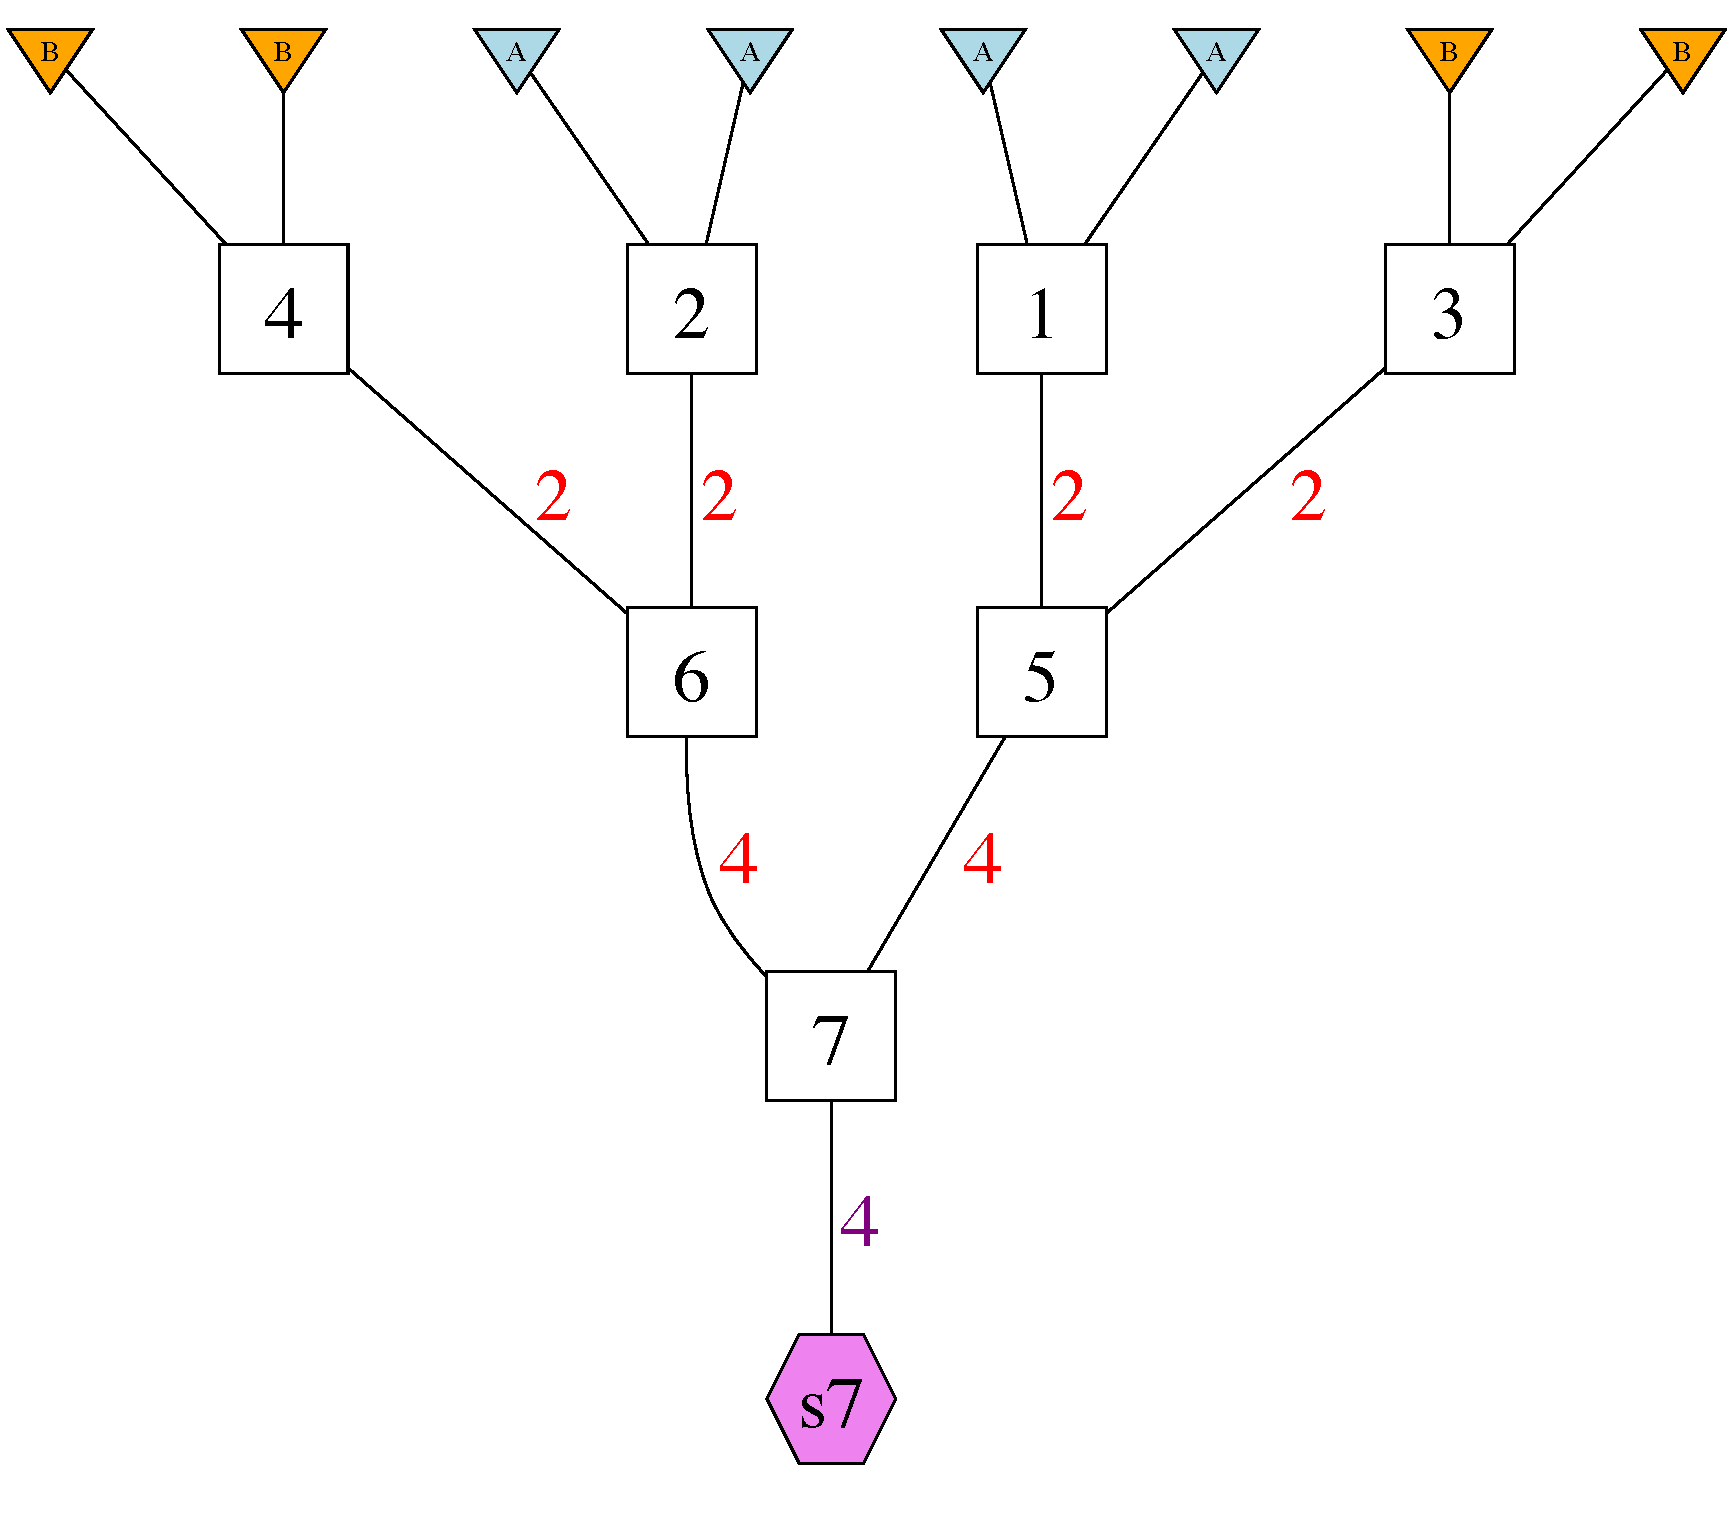
\includegraphics[width=\columnwidth]{figures/F2.pdf}
\end{center}
\caption[\gspcapone]{\gspcapone}
\label{fig:gsp1}
\end{figure}
%%%%%%%%%%%%
%%%%%
\begin{figure}
\newcommand{\gspcaptwo}{\footnotesize
An example GSP generated by {\footnotesize\tt create\_GSP()} that produces four different
admixture categories: one~$F_1$ in sample node~s7; two~$F_2$'s in sample node~s11; one $\BC_1$ in sample node~s9; and two $\BC_2$'s in sample node~s10.
}
\begin{center}
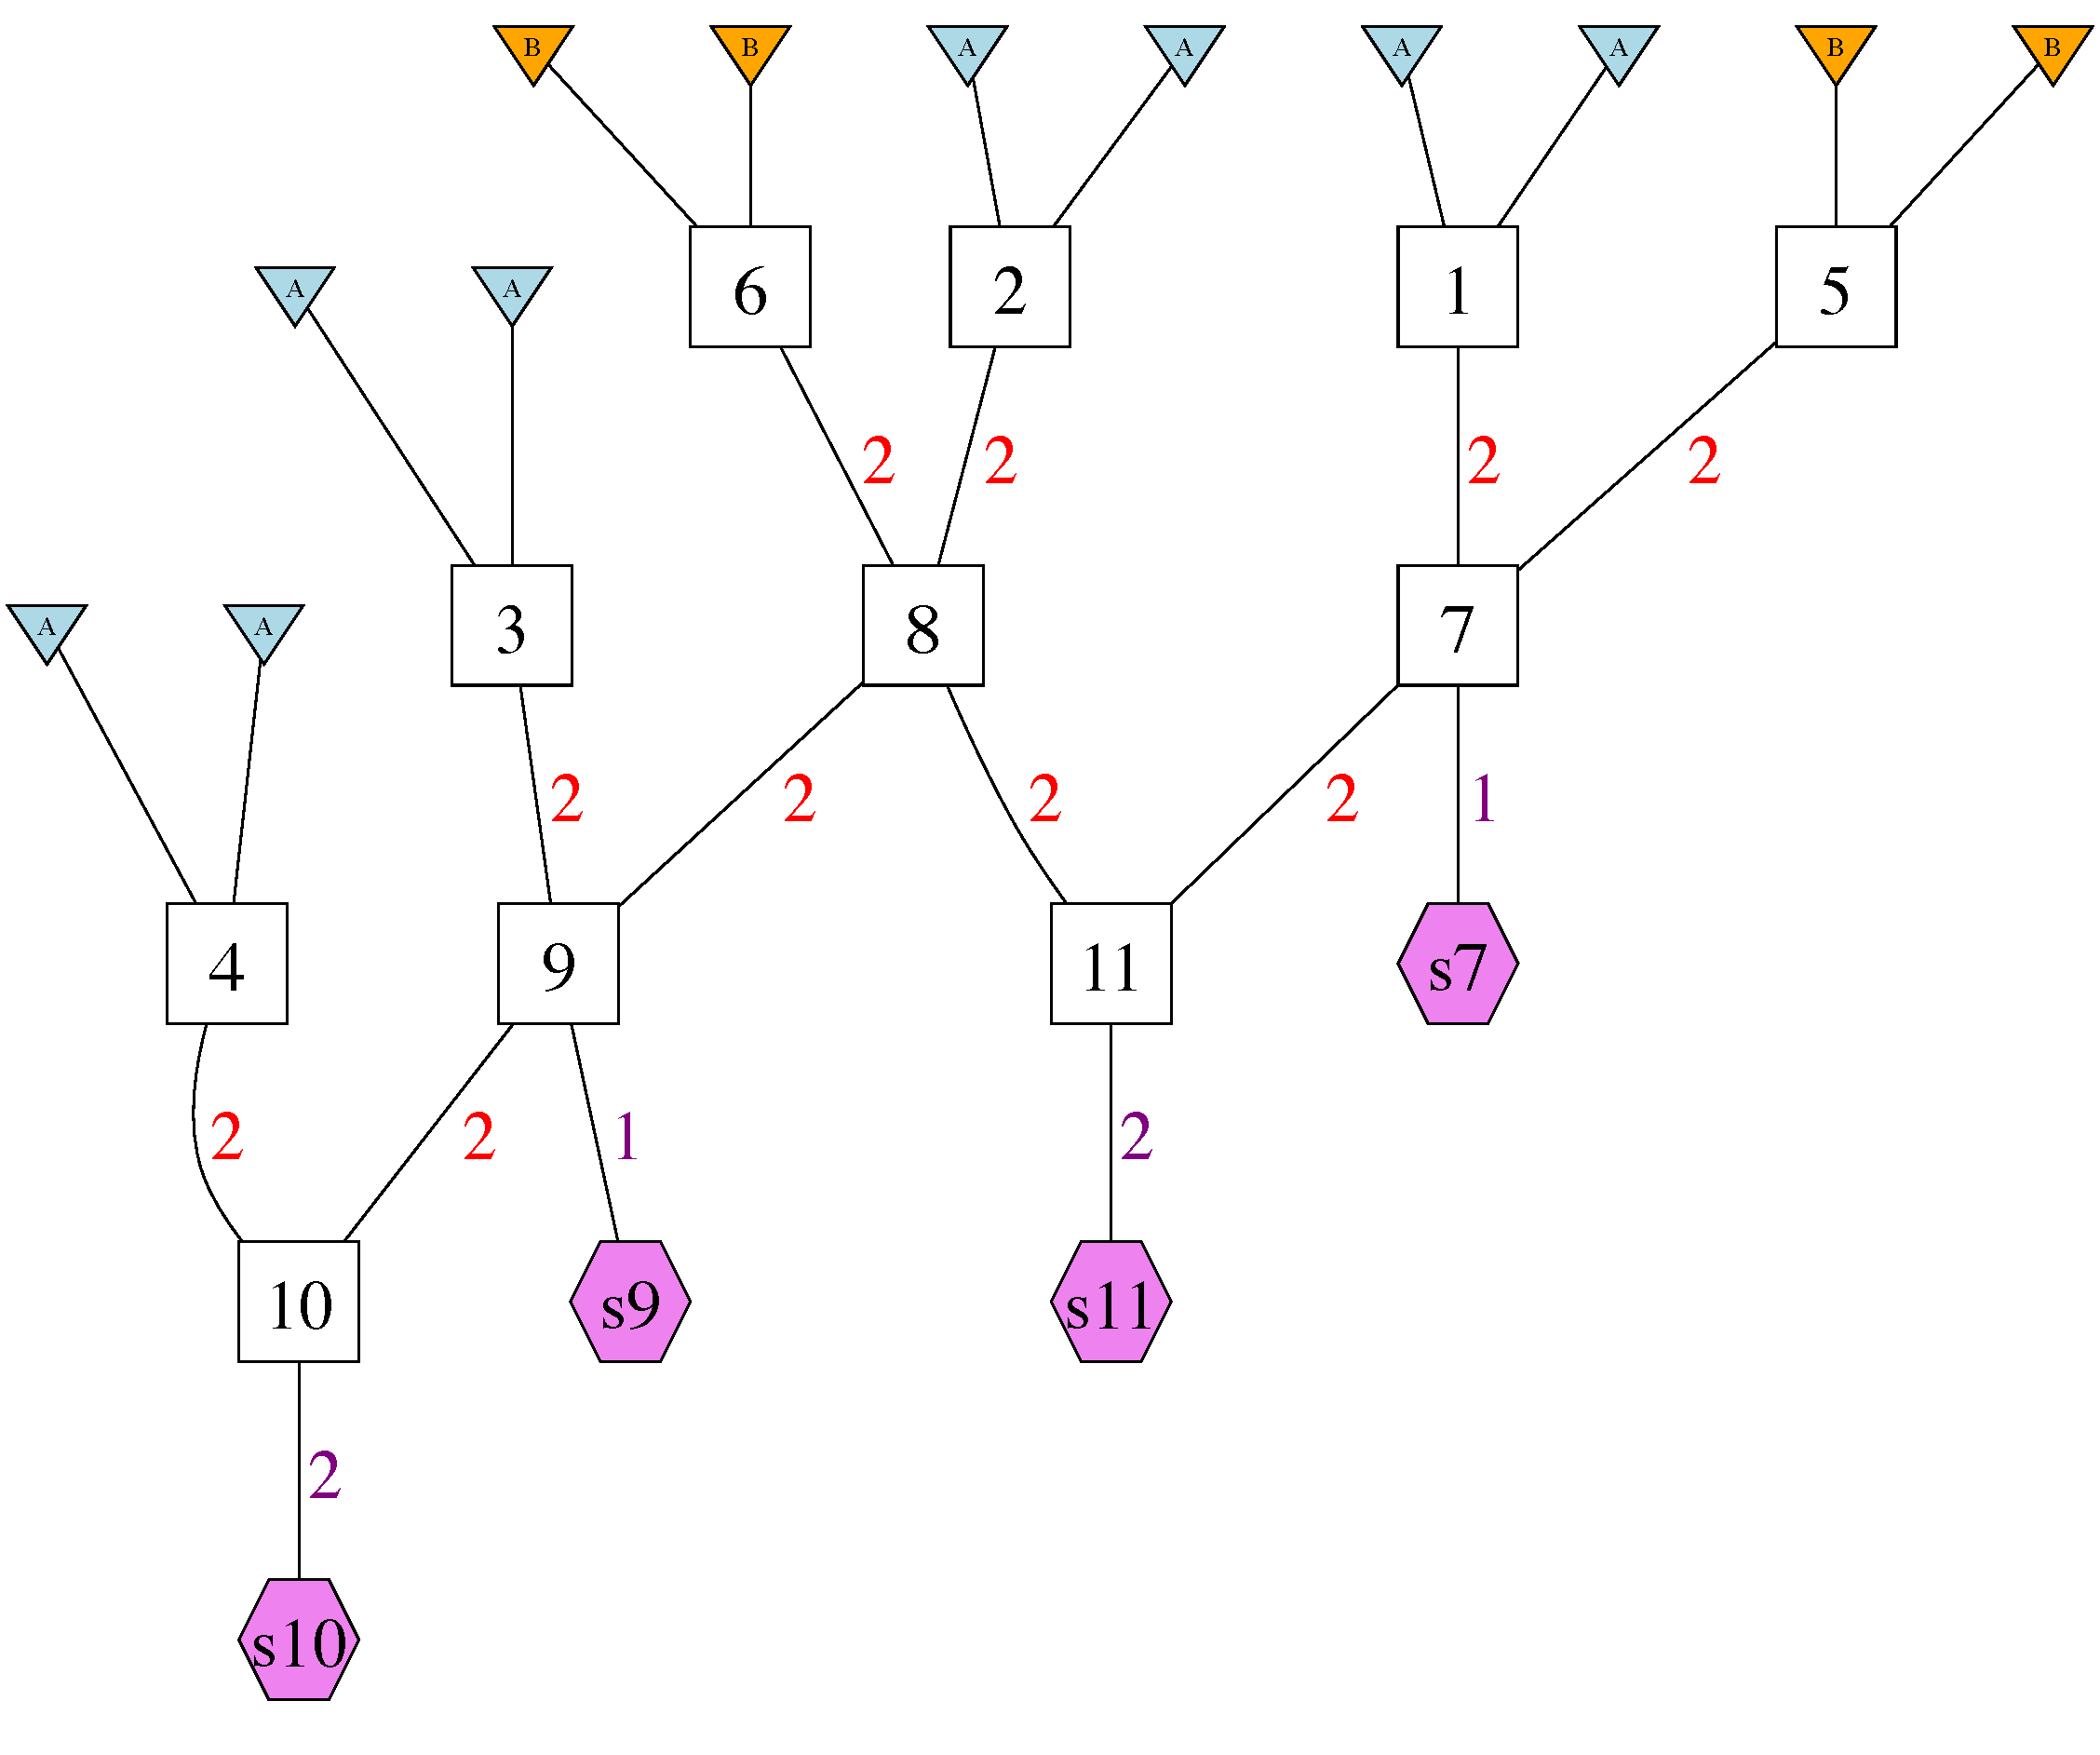
\includegraphics[width=\columnwidth]{figures/AllThem.pdf}
\end{center}
\caption[\gspcaptwo]{\gspcaptwo}
\label{fig:gsp2}
\end{figure}
%%%%

{\sc hybridlab} was conceived at a time when
the data sets used in molecular ecology universally included very few markers, such that
it was reasonable to assume the markers were unlinked, and, hence, independently segregating.
Today, however, with data sets of thousands of markers, that assumption is badly violated---alleles
on the same chromosome are likely to be segregated together into the next generation.
Simulating linked loci as independent creates simulated hybrids, beyond the $F1$ category, with 
artificially low variance in admixture fraction, leading to the false interpretation that different
hybrid categories are more easily distinguished than they are. Therefore, in evaluating descendants of migrants within a simulated framework, it is imperative to take into consideration the pattern of
linkage among loci available for analysis. This was done recently to assess the power of a SNP panel for identifying descendants of escaped, farm-raised Atlantic salmon \citep{wringe2019development}; however the method used (described at https://eriqande.github.io/SalarHybPower/) was developed in an {\em ad hoc} fashion, was not easily extended to
complex hybridization scenarios, and was not at all user-friendly.

In response to these needs, we developed \gscramble{} – a simulation approach that samples alleles from respective populations without
replacement, thus maintaining genetic differences between the clusters commensurate to those in the empirical dataset, and eliminating the effect of RISPI.
Further, by simulating individual genotypes based on user-defined pedigrees of arbitrary complexity, \gscramble{} allows for the simulation of admixed genotypes resulting from any conceivable category of hybrid, while allowing the tracking of haplotype blocks from source populations within the specified pedigree.
By integrating species-specific recombination rates, \gscramble{} simulates biologically informed genotypes that mirror empirical data.
We develop and illustrate \gscramble{} with use of single nucleotide polymorphic (SNP) genotypes, though it is equally applicable to data sets with hundreds or thousands of
microhaplotypes \citep{baetscher2018microhaplotypes} or microsatellites
\citep{zhan2017megasat}.




\section*{Methods}

\subsection*{Two introductory motivating examples}


Before we proceed to a description of the methodology used by \gscramble{},
we demonstrate two important points through two simple simulations.  In the first,
we show that using a standard sampling-with-replacement
approach induces RISPI when estimating admixture fractions. In the second, we show
the effect of physical linkage on the distribution of admixture fractions of hybrid individuals,
which vividly shows why it is not acceptable with large numbers of markers, to simulate
the genotypes of hybrid individuals assuming no physical linkage.


\subsubsection*{RISPI when estimating admixture fractions}
\label{sec:rispi-sim}

To construct this simple example, we used the R programming language \citep{Rcoreteam} to
simulate allele frequencies for $L$ biallelic
loci in a single population from a $\mathrm{Beta}(1, 8)$ distribution and then simulated
two samples, $A$ and $B$, each of size $N$ diploid genotypes. The genotypes in $A$ and $B$ were simulated
from the same allele frequencies assuming Hardy-Weinberg equilibrium.

In this case,
each set of $N$ individuals is a sample from exactly the same population, so
there is clearly no basis for performing population assignment between $A$ and $B$;
however, we treated samples $A$ and $B$ as if they were sampled from two potentially different
populations, and simulated $9n$ new individuals: $n$ new individuals at each of the 9 values of
$q_A$, the admixture fraction for population $A$, in  $\{0, \frac{1}{8}, \frac{1}{4}, \frac{3}{8}, \frac{1}{2}, \frac{5}{8}, \frac{3}{4}, \frac{7}{8}, 1\}$.
We simulated these genotypes according to the "admixture model" used in {\em structure} \citep{pritchard2000inference}.  Briefly, at each
locus, independently, the origin
of each gene copy was simulated to be from
population $A$ with probability $q_A$ and from population $B$ with probability $1-q_A$.  Subsequently,
the allelic types of gene copies from $A$ ($B$), at a locus, were simulated by sampling with replacement
from the alleles at that locus in sample $A$ ($B$).
We then added these $9n$ simulated individuals to the $N$ original individuals  from $A$ and $N$ from $B$
and analyzed all the genotypes using ADMIXTURE with $K=2$. On each data set we performed a supervised analysis in which the original
$N$ samples from each
population were provided as learning samples, and also an
unsupervised analysis when the origin of the samples from $A$ and $B$ were regarded as unknown.

For each combination of $L \in \{10^2, 10^3, 10^4, 10^5\}$,
$N \in \{25, 50, 100, 250\}$ and $n\in\{3,12,24\}$ we conducted multiple replicates
of the entire process of
simulating samples $A$ and $B$, simulating the $9n$ additional individuals, and
then analyzing them with ADMIXTURE.  We conducted $R$ replicates so that,
for each combination of $L$, $N$, and $n$ we had simulated $Rn=480$ new individuals
at each $q_A$ value; thus, $R=160$ replicates when $n = 3$, $R=40$ when $n=12$, and
$R=20$ when $n=24$.


Because the simulations were done in a na\"{i}ve way that effectively assumes that the population
allele frequencies are identical to those observed in the samples themselves, we hypothesized that ADMIXTURE would return estimates of
$q_A$ that were
centered around the simulated values, even though samples $A$ and $B$ were drawn from the same
population. In other words, we expected to observe RISPI.
We further expected that ADMIXTURE would return more accurate estimates of the simulated
$q_A$ values when $N$ was smaller and the number of loci was larger.
We summarized the results by plotting boxplots of the ADMIXTURE-inferred $q_A$ values,
 for the 480 newly simulated individuals (and for the original samples, $A$ and $B$, in the
 case of unsupervised clustering),
for each combination of $L$, $N$, and $n$.

%NOTE, WE ALSO DID THESE SIMULATIONS USING GSCRAMBLE AND WE COULD NOTE
%HOW THOSE CAME OUT.  
% BUT MAYBE JUST HAVE THAT IN CASE A REFEREE ASKS ABOUT IT.



\subsubsection*{Physical Linkage in Hybrid Individuals}

We first simulated the genotypes of hybrids between two species, $a$ and $b$,
considering $F_2$'s and first- through
fourth-generation backcrosses in each direction, erroneously treating each
locus as if it were independently segregating (as done, for example, in {\sc HybridLab}). Thus,
each locus independently is simulated to have a genotype of 2, 1, or 0 gene copies originating from species $a$ [{\em e.g.}~genotypes of $(a,a)$, $(a,b)$, or $(b,b)$] according to the expected
probability of each genotype given the hybrid category (see \citealt{anderson2002model}).
48,000 hybrids were simulated at each number of loci, $L$, in $\{10^2, 10^3, 10^4, 10^5\}$.
The admixture fraction of each simulated individual was recorded as the fraction of all $2L$
gene copies originating from species $a$.  

We also simulated the genomes of 48,000 individuals of each
hybrid category using \gscramble{}'s {\footnotesize\tt segregate()} function, as described
below, with number of chromosomes and sex-averaged recombination rates
for pigs, as estimated by from \citet{tortereau2012high}. In this case, we recorded the
admixture fraction of each simulated individual as the fraction of all genome segments
that originated from species~$a$.  This provides the distribution of the true admixture fraction
when physical linkage of markers is not ignored.  

All the admixture fraction distributions were summarized by plotting them as histograms
so they could be compared easily.  


\subsection*{Genomic Simulation Pedigrees}

Our approach for simulating admixed individuals without creating RISPI is motivated by the traditional cross-validation
approach for evaluating the power of mixture proportion
estimation in genetic stock identification (e.g., the cross-validation approach
described in \citealt{moran2019bayesian}).
In the cross-validation approach, individuals are removed from the reference
samples and placed in a mixture sample of "unknowns", whose origin
is inferred using the remaining individuals in the reference samples.  A key
feature of this approach is that no new genetic material is being created by
sampling with replacement; rather the genetic material of all individuals
in the original sample is being used---either within the remaining individuals in the
reference samples or within the individuals in the mixture.

Our scheme, described here, extends the traditional cross-validation approach
by simulating the descent of chromosomal linkage blocks through a user-specified
pedigree to create admixed individuals.  By imposing certain constraints
on the pedigree, our framework ensures that all the genetic material
within the original individuals is used to either create admixed individuals or is retained
within reference individuals (i.e., those that are purely of one
putative subopulation), and yet no new genetic material is
created by sampling with replacement from the original samples.

We refer to the structure used to implement this cross-validation simulation
of admixed individuals as
a {\em genomic simulation pedigree} or GSP.  Like any pedigree,
a GSP includes a set of founders (individuals that have no parents specified in the
pedigree), and it includes non-founders; however, we introduce an additional node
type in the GSP that represents samples taken from the non-founders. These samples
are the simulated admixed individuals.  A GSP must have no inbreeding loops, since
any inbreeding loop indicates that more than one copy of a gene in an ancestor may
be created amongst its descendants, which is a type of sampling without
replacement.  Furthermore, in a GSP, the amount of genetic material taken from the
samples at the sample nodes should be equal to the amount of material in the founders,
to ensure that all available data is being used to estimate power for the estimation of
admixture fractions.

Figure~\ref{fig:gsp1} shows an example GSP for the simple case
of simulating $F_2$ individuals. The figure and its caption
should be studied, as the following section
uses terminology that is defined in the figure caption.

It is important to understand that, apart from the founder nodes, the individual
nodes in a GSP do not necessarily represent only a single individual.  Specifically,
since we are preserving all genetic material, multiple gametes may get segregated
through each non-founder node in a GSP\@.

Genetic material is segregated through
a GSP using these steps, done upon each node in an order such that the steps
are run on each node's parents before being run on the node itself:
\begin{enumerate}
\item Each genome in a triangle above a founder node represents a gamete
carrying a single, haploid copy of the genome.
These gametes are united within the founder individual and then
recombination occurs between each chromosome
with probability $\frac{1}{2}$ and within each chromosome according to
a user-specified recombination map to create two new gametes, which are
recombined versions of the original ones.  These two gametes are then segregated at random down the edge (or edges) from the founder node. Upon each edge, $i$ from founder node $f$, $G^-_{f,i}$ gametes are segregated. 
\item Each non-founder node, $x$, will have exactly two edges coming
into it---one from each parent.  Each of the $G^+_{x,1}$ gametes coming in from the
first edge is united with a single one of the $G^+_{x,2}$ gametes coming
in on the second edge (in a random order).
\item If a non-founder node $x$ has an edge to a sample node,
a randomly chosen $S_x$ of the united pairs of gametes are delivered
to the sample node to constitute the $S_x$ samples taken from individual
node $x$. Any remaining united pairs of gametes are treated as in (4) below.
\item United pairs of gametes (including those remaining after delivery
to a sample node) in each non-founder node $x$ are segregated into
gametes with recombination, and each of these gametes is assigned, in
random order, to the gamete edges proceeding downward out of the node,
with the number of gametes assigned to the $i\thh$ downward edge being
$G^-_{x,i}$.
\end{enumerate}
At the end of this process, the samples simulated (as united pairs of gametes)
into the sample nodes will contain all of the genetic material (and no more) found among the founders, but that
material will have been segregated and recombined according to the pedigree.  Thus the
samples obtained from a GSP can be simulated with the expected admixture fractions
for any hybrid category that can be specified by a pedigree.  They have also been simulated
in a way that 1) reflects physical linkage---each individual inherits segments of the genome
simulated using a recombination map; 2) does not duplicate any genetic material---the sampling of
genetic material is entirely without replacement so it will not induce RISPI; and 3) no genetic material has been lost---all the genetic material of the founders
is represented in the samples, maximizing the number of simulated individuals and markers available to
use in downstream analyses.

In the \gscramble{} package there is a convenience function called {\footnotesize\tt create\_GSP()} that
will create GSPs for samples up to and including second-generation backcrosses (an example appears in Figure~\ref{fig:gsp2});
however, \gscramble{} is designed
to handle user-specified GSPs of arbitrary complexity.  When creating a unique GSP,
the following requirements are necessary for the GSP to be valid
and the simulation to execute successfully.
Writing $\founders$ for the set of all founder nodes, $\nonfound$ for the set of all non-founder nodes, and $\nonfounds$ for all non-founder
nodes that are not parents of other non-founders, but are adjacent to a sample node, $\nonfounde$ for all
non-founder nodes that have non-founder node daughters, but no sample nodes, and $\nonfoundse$ for all
non-founder nodes that are parents of non-founder nodes and also adjacent to sample-nodes, the necessary conditions
for a valid GSP, in addition to having no inbreeding loops, are:
\begin{equation}
\begin{aligned}
\sum_{x \in \nonfounds \cup \nonfoundse} S_x &= |\founders| &  \\
\sum_{i=1}^{e_x} G^-_{x,i} &= 2 & \forall x \in \founders \\
G^+_{x,1} &= G^+_{x,2} & \forall x \in \nonfound \\
\sum_{i=1}^{e_x} G^-_{x,i} &= G^+_{x,1} +  G^+_{x,2} & \forall x \in \nonfounde  \\
 S_x/2 + \sum_{i=1}^{e_x} G^-_{x,i} &= G^+_{x,1} +  G^+_{x,2} & ~~~\forall x \in \nonfoundse.  \\
\end{aligned}
\end{equation}
Before simulating from a GSP, \gscramble{} checks to ensure the GSP
satisfies these validity conditions.  The simulation of genomic segments
from founders to samples in a GSP is performed by the \gscramble{} function
{\footnotesize\tt segregate()}, which requires as input a list of GSPs through which
to segregate genomic segments, and, for each such GSP, a table that maps the
population labels on each GSP (in the inverted triangles atop the founders) to the
different sampled groups of individuals.

\subsection*{Permutation procedures}

\gscramble{} uses a GSP to segregate segments of genetic material from the founders
to the samples.  At the end of segment simulation, the genome of each sample
is recorded as a mosaic of segments that derive from different founders.  In order
to create a data set of markers in each sample, it is necessary only to identify the alleles
that occurred on each segment within the founders and propagate those alleles to the
corresponding segments within the samples.  At the stage of assigning alleles to
founders, \gscramble{} provides a variety of ways to permute alleles amongst
the collection of individuals from which the founders are drawn.  By using permutation,
variability in the data is created, but, since it is done without sampling with replacement, it does
not induce RISPI.

%%%%%%%
\newcommand{\permcap}{\footnotesize An illustration of how \gscramble{} permutes data under
different options.  {\bf (a)}~A picture
representing an original data set of $N=12$ diploids sampled from three populations and typed at $L=15$ markers.
Different colors represent different sampled individuals. Individuals 1--5 are shades of blue and green, indicating that they
are from a single population.  Individuals 6--9 are from another population, (shades of red and orange), while 10--12
are from a third population and are colored shades of violet. Thick vertical black lines separate the different
populations.  Markers are shown in rows. There are 6 markers on the first chromosome, 5 on the second, and 4 on the
third.  Each chromosome is delimited by a thick, horizontal black line. The "a" and the "b" in the colored cells denote the first and second gene copies within an individual at each marker.  It is worth noting that this representation shows a $2L \times N$ matrix,
which is the transpose of the $N\times 2L$ matrix used to supply genetic marker data to \gscramble{}. {\bf (b)}~Examples of how the {\tt\footnotesize preserve\_individuals} and {\tt\footnotesize preserve\_haplotypes} options of the {\tt\footnotesize segments2markers()}
function affect the permutation of
the genetic data of the original data set.  Panel headers show the option values while the colors and "a" and "b" values
in the colored cells show the original position of each gene copy in the original sample.  Note that permutation is always
done within the populations.  When {\tt\footnotesize preserve\_individuals = TRUE},  then just the
individuals in their entirety are permuted.  When {\tt\footnotesize preserve\_individuals = "BY\_CHROM"}, each pair
of a single chromosome within an individual remains together when permuted. When {\tt\footnotesize preserve\_individuals = FALSE}, gene copies are freely permuted between individuals.  The option {\tt\footnotesize preserve\_haplotypes = TRUE} causes each haplotype on a chromosome to be preserved
while permuting. This option should only be used when the original data set is phased.
}
\begin{figure*}
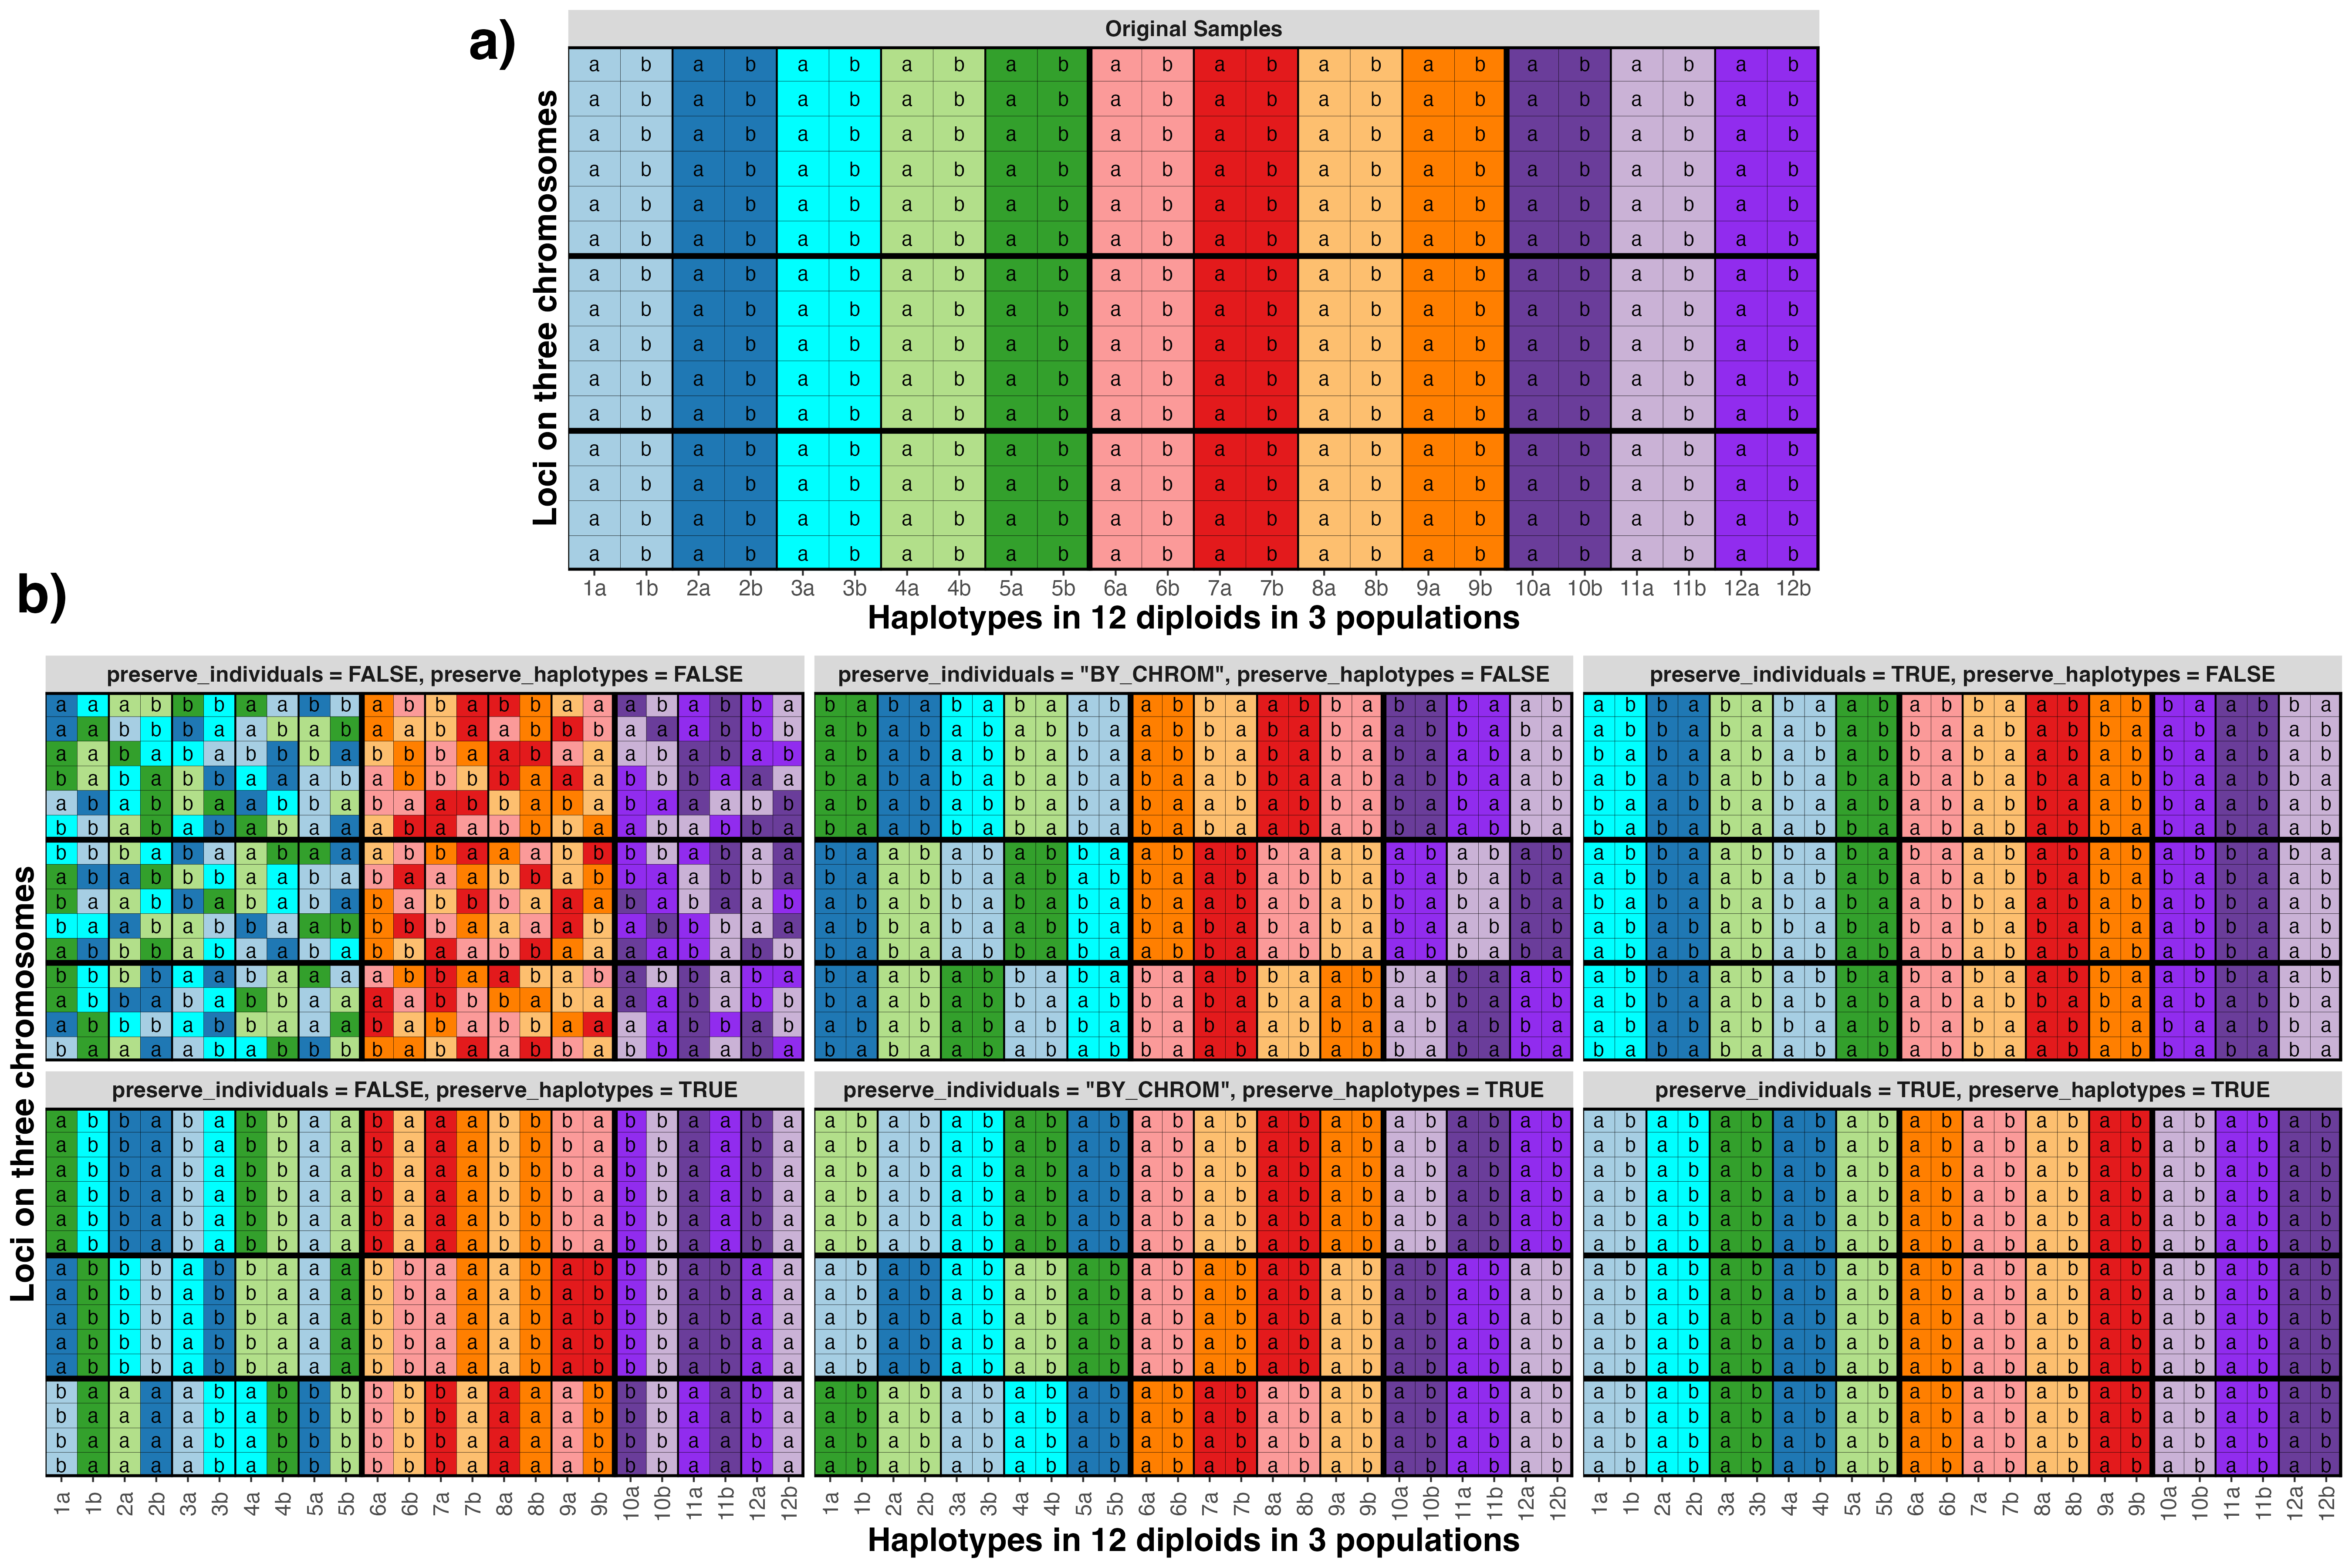
\includegraphics[width=\textwidth]{figures/permutations-plot.png}
\caption[\permcap]{\permcap}
\label{fig:perms}
\end{figure*}
%%%%%%%



These permutations are implemented with the genotypes provided by the user.
\gscramble{} accepts genetic data as a matrix with $N$ rows (one for each individual) and
$2L$ columns (two for each locus). If the data have been phased, then the phased alleles from the
first haplotype should occupy the
first entry for each locus within an individual, while alleles phased together on the second haplotype should occupy the
second entry for each locus.
There can be several populations represented in the data set, but
each individual must belong to exactly one
population.

Permutation of alleles proceeds within populations, such that
the frequencies of alleles from each population remain the same as those observed
in the samples themselves. Following permutation, there remain individuals
in each population, but the alleles that they carry are different after permutation.  These
individuals are assigned, in order, to be the founders from each population in the GSP. Subsequently,
after genetic material is segregated to the samples, the alleles found on each genomic segment in those permuted
founders are then propagated to the samples.  It is worth noting that this approach allows for simulation
with large genomic data sets, with hundreds of thousands to millions of markers, since segregation
through the pedigree is done by segments, and not on a locus-by-locus basis. The only operations
involving all the alleles in all the individuals are the permutation steps and indexing into the segments,
which may be done efficiently with matrices in R.

Permutation of alleles is handled within the \gscramble{} function {\footnotesize\tt segments2markers()}
which takes as input the segments segregated down a GSP, a matrix of sampled genotypes, and a specification
of the group that each sampled individual belongs to.  The permutation performed when running
{\footnotesize\tt segments2markers()} is controlled by two main options.  The first, {\tt\footnotesize preserve\_individuals},
can take three different values.  If {\tt\footnotesize preserve\_individuals = TRUE}, then entire individuals are the unit that gets permuted within the
data set,
such that all the alleles within an individual remain together.  If {\tt\footnotesize preserve\_individuals = "BY\_CHROM"}, then
the alleles within an individual found on a homologous pair of chromosomes remain together, but the different
chromosome pairs of an individual are independently permuted into new positions in the data set.  This form of permutation
maintains the linkage disequilibrium (LD) between markers on the same chromosome, which may be desirable in some contexts.
If {\tt\footnotesize preserve\_individuals = FALSE} then each gene copy within an individual is permuted separately,
providing the maximal scrambling of the data. The second option, {\tt\footnotesize preserve\_haplotypes}, can take two
different values, {{\tt\footnotesize FALSE} (the default) and {\tt\footnotesize TRUE}.
This option, which keeps alleles together
on the same haplotype, should be set to {\tt TRUE} only
if the original genotypes have been phased into separate haplotypes.
Fig.~\ref{fig:perms} depicts, graphically, the effect of using different settings of
{\tt\footnotesize preserve\_individuals} and 
{\tt\footnotesize preserve\_haplotypes}, together.


% I THOUGHT ABOUT PUTTING THESE RESULTS IN, BUT I
% THINK WE ARE FINE WITHOUT THEM.
%\subsection{Simulation: \gscramble{} Eliminates RISPI}
%
%We present a brief simulation similar to those in
%section ``RISPI when estimating admixture fractions,'' but conducted using
%\gscramble{} rather than sampling with replacement.  We focused on two
%scenarios that 

\subsection*{Examples}

We illustrate the use of \gscramble{} in three example cases. The first is
a simple simulatino to show that, unlike sampling with replacement, the
approach of \gscramble{} does not produce RISPI.
The next two are examples using empirical data sets.
The first of these involves
simulating a small number ($<\,$70) of markers that are fixed, or nearly
fixed, for alternate alleles between two species of trout: rainbow trout ({\em 
Oncorhynchus mykiss}) and cutthroat trout ({\em O. clarkii}). The goal of the 
simulation study is to determine how accurately individuals of different hybrid
categories between the species can be identified, and whether the use of linked 
markers deflates the estimates of uncertainty to an unacceptable degree.  The 
second example involves many more markers ($\approx$14,000) and 
investigates the accuracy for
identifying individuals admixed between closely related groups of feral
pigs in Missouri.  

\subsubsection*{No RISPI when using \gscramble{}}

For this example, we repeat the simulation described in \nameref{sec:rispi-sim};
however, after simulating individuals in the two samples drawn from the same population,
we create data sets of admixed individuals using \gscramble{}, rather than sampling
gene copies with replacement.  As before, individuals were simulated with fractions of
ancestry from sample $A$ in $\{0, \frac{1}{8}, \frac{1}{4}, \frac{3}{8}, \frac{1}{2}, \frac{5}{8}, \frac{3}{4}, \frac{7}{8}, 1\}$, but these were simulated from pedigrees using gscramble.  We limited
this simulation to one of the scenarios that showed extreme RISPI when sampling gene
copies with replacement: $L=1,000$ markers with sizes of samples $A$ and $B$ being
$N=50$. This simulation was repeated 240 times, and the results of each analyzed with
ADMIXTURE to estimate the ancestry fractions of each simulated individual.

\subsubsection*{Rainbow/cutthroat trout hybrids in California}

We used the archived data from \citet{rizza2023limited}, drawing upon their 65 markers
that are fixed or are nearly fixed for alternate alleles between rainbow trout and cutthroat trout.
They designated 634 fish as pure cutthroat trout and 213 as pure steelhead.  We used the
genotypes of these individuals as input to \gscramble{}.

\citeauthor{rizza2023limited} mapped the 65 markers to the Omyk\_v1.0 genome assembly (RefSeq 
Accession: GCF\_002163495.1), so we used
the linkage map described in \citep{pearse2019sex} that was prepared by linkage mapping 
of $\approx$57,000 markers described in \citet{palti2015development} to Omyk\_v1.0. We mapped the $\approx$57,000 markers to Omyk\_v1.0, and then resolved inconsistencies to produce a map
of 32,923 markers throughout the genome and rendered it to plink format for use with \gscramble{}.

In the original paper, \citet{rizza2023limited} identified 15 $F_1$s,
1 $F_2$,
6 cutthroat backcrosses ($BC1$s) and 
6 second-generation cutthroat backcrosses ($BC2$s),
and 1 fish of an unknown hybrid category that may have been the
product of a $BC2$ crossed with a $BC1$.   In our simulations, we sought to simulate
a similar collection of hybrid individuals, so, for each replicate, we used
\gscramble{} to simulate 16 $F_1$s, 4 $F_2$s, 6 $BC1$s, 4 $BC2$s, 4 $BC3$s,  4 individuals
that were the products of a $BC1$ mating with a $BC2$, and finally, 4 individuals that were simulated pure cutthroat. Individuals not used as founders
in \gscramble{} were retained as pure cutthroat and pure steelhead.  The goal of the simulation
was to assess how well these different hybrid categories can be distinguished from one another
when using either all 65 markers, or just the 30 markers occurring on different chromosome arms
used by  \citet{rizza2023limited}.

We performed 500 replicate simulations with \gscramble{} using either 30 or 65 markers.  Each
simulated data set was then analyzed using {\sc NewHybrids} \citep{anderson2002model}. Individuals not used as founders were given the ``s'' and ``z'' flags, indicating that they were considered training samples.  The remaining 46 individuals were treated as possible hybrids and their genetic data used to calculate the posterior probability that they belonged to one of 10 hybrid categories as shown in Table~\ref{tab:newhybcats}, using 25,000 MCMC sweeps and discarding the first 5,000 as burn-in.
%%%%%%%%%%%%
\begin{table}
\caption{The 10 hybrid categories considered for inference with {\sc NewHybrids} and the
expected frequency of their genotypes having 2 ($f(C,C)$), 1 ($f(C,S)$) or 0 ($f(S,S)$) copies of ancestry from cutthroat trout.}
\label{tab:newhybcats}
{\small
\begin{tabular*}{\columnwidth}{@{\extracolsep{\fill}} lrrr}
\hline\hline
Category	& $f(C,C)$ &	$f(C,S)$ & 	$f(S,S)$ \\ \hline
\input{inputs/newhybs-cats.tsv}
\end{tabular*}
}
\vspace*{-2.3ex}\hrule\vspace*{0.3ex}\hrule
\end{table}
%%%%%%%%%%%%



\subsubsection*{Invasive wild pigs in Missouri}

Genetic samples were collected from 160 invasive wild pigs in southeastern
Missouri that were lethally removed through population control efforts
conducted as a component of the Missouri Feral Hog Elimination Partnership
by US Department of Agriculture – Animal Plant Health Inspection Services –
Wildlife Services, Missouri Department of Conservation, and other cooperative
federal and state agencies.
DNA was extracted from hair or tissue (collected from animals at the time of euthanasia) with
commercially available magnetic bead recovery kits (MagMax DNA, Thermo Fisher Scientific).
Genotyping was performed with GeneSeek’s Genomic Profiler for Porcine HD which provides
62,128 biallelic SNP loci that are mapped across the 18 autosomal chromosomes.
We implemented standard genotype quality control measures; specifically, we pruned loci with
call rates $<95\%$ and minor allele frequencies $<5\%$.
We implemented linkage disequilibrium (LD) pruning using a window size of 50 loci and step size
of 5 loci to remove markers above a linkage threshold of $R^2 > 0.5$.

The 160 invasive wild pig samples represented 120 reference individuals from the core regions of
3 populations (40 individuals each informed by previous analyses)
and 40 individuals from the contact regions of these populations.
We used ADMIXTURE version 1.3.0 \citep{alexander2009fast} to characterize the genetic structure
of the 160 samples (for $K = {1...6}$). Using the 120 reference individuals identified to represent population cores,
we sought to classify the admixture patterns of the 40 empirical samples
from the contact regions using simulated pedigrees from \gscramble{}. To address this objective we simulated
pedigrees to represent the likely classes of admixed individuals that would be present in the samples
from the contact regions of the 3 reference populations. The types of admixed individuals we considered were
$F_1$, $F_2$, $\BC_1$ and $\BC_2$ representing all two-population combinations
(Pop1 x Pop2, Pop1 x Pop3, Pop2 x Pop3, and reciprocally Pop2 x Pop1, Pop3 x Pop1, Pop3 x Pop2 as required
to simulate backcrossed classes).
We also simulated individuals from each of the founder populations. The first step of this workflow involved
simulating admixed individuals for 2 founder populations using one of the preset \gscramble{}
GSPs provided by the function {\footnotesize\tt create\_GSP()} for producing each of the types of admixed
individuals. Although we could have simulated all 4 types of admixed individuals from a single GSP (Figure~\ref{fig:gsp2}),
different numbers of simulated individuals are produced for each hybrid class. Therefore, for the sake of the
computational efficiency from simulating the exact number of desired individuals, we chose to simulate from
a single GSP for each of the hybrid classes by setting the corresponding hybrid parameter in {\footnotesize\tt create\_GSP()} to {\footnotesize\tt TRUE}. We used the default settings of the {\footnotesize\tt plink\_map2rec\_rates()} to specify the recombination rates. The 120 simulated genotypes were written to PLINK .ped and .map files using {\footnotesize\tt gscramble2plink()}. We used PLINK version 1.9 \citep{purcell2007plink} to convert the genotypes to binary files and used these as input into ADMIXTURE for which we specified $K=3$ to produce ancestry values. We iteratively
performed this workflow to produce 1,000 simulated genotypes and ancestry values for each of the
4 hybrid classes, as well as founder individuals, for each of the population combinations, for a total of
21,000 simulated individuals.

\section*{Results}

\subsection*{Two Introductory Motivating Examples}

\subsubsection*{RISPI when estimating admixture fractions}

As expected, the perceived ability to estimate $q_A$ with ADMIXTURE was higher
for larger values of $L$ and for smaller values of $N$ (Figure~\ref{fig:bias-sims}).
%%%
\begin{figure*}
\newcommand{\biassimscap}{\footnotesize ADMIXTURE estimates of $q_A$ as described in
{\em An introductory motivating example}. In these results, the apparent ability to estimate $q_A$
is a bias resulting from the use of sampling with replacement to simulate new, admixed genotypes to
test in ADMIXTURE.  In each figure, the different columns represent different numbers of markers
from 10 to 100,000, while different rows represent different original sample sizes, $N$, taken. Colors
of the boxplots indicate how many new individuals, $n$, of each $q_A$ value were simulated during each
replicate.}
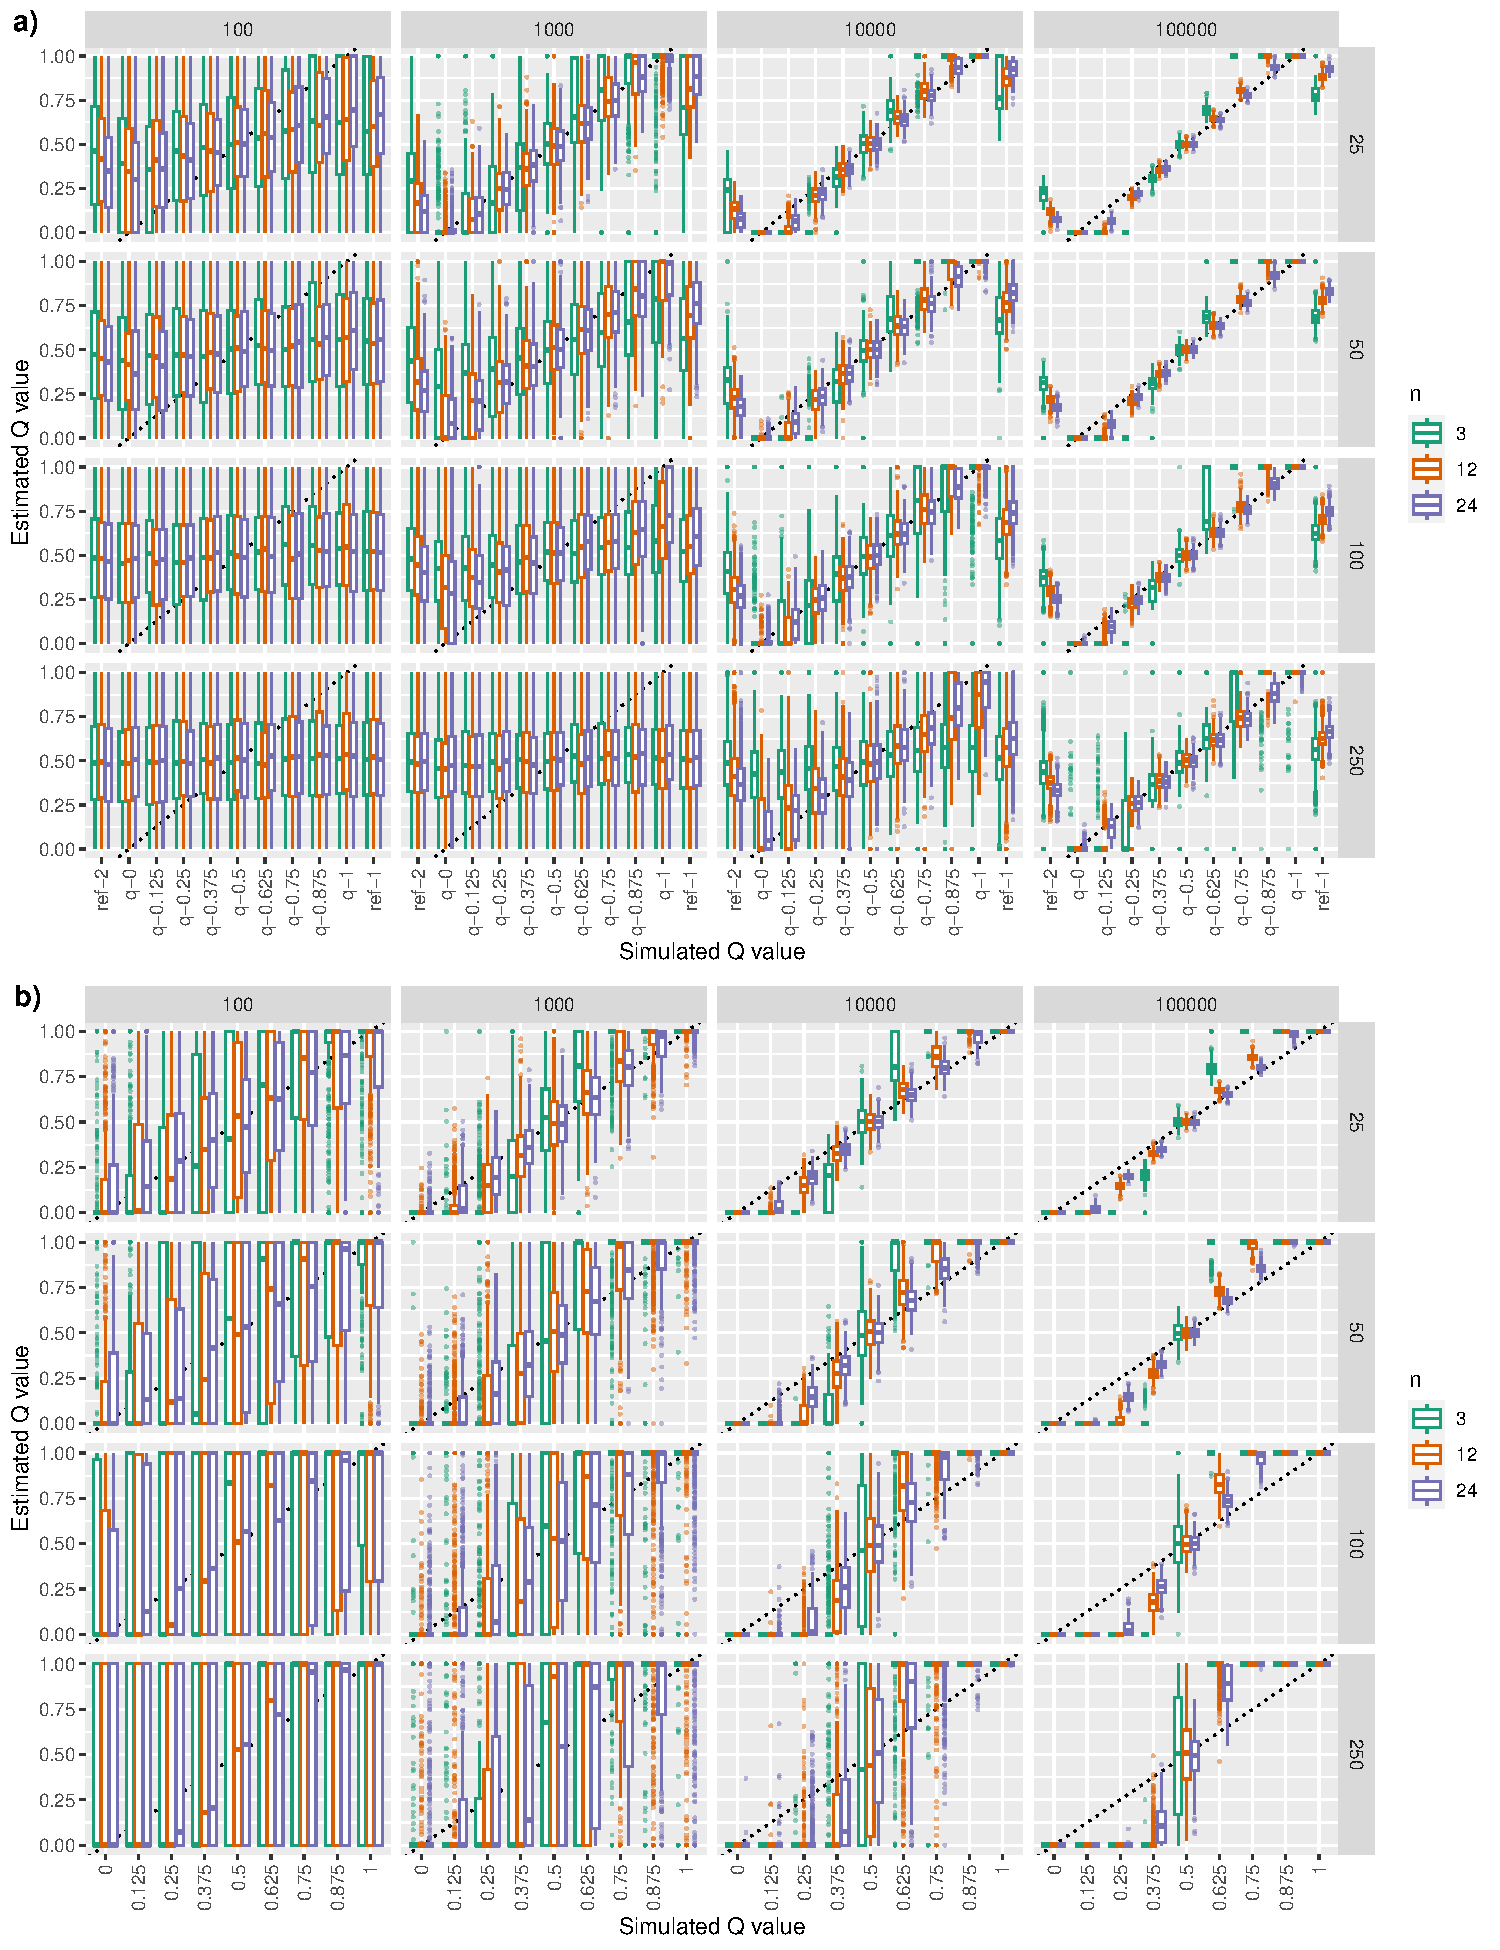
\includegraphics[width=0.96\textwidth]{figures/bias-sims-unsup-and-sup.pdf}
\caption[\biassimscap]{\biassimscap}
\label{fig:bias-sims}
\end{figure*}
%%%
It is interesting to note
that, for numbers of loci,  $L$, that are 100 (or smaller) the effect is observed only when
sample size, $N$, is as small as 25---and even then the effect is slight.  However, when the
number of markers increases to 100,000---values that are becoming commonplace with the availability of chip-
or sequencing-based approaches---it is apparent that the sampling-with-replacement approach
induces an extreme bias.  With 100,000 markers, even if sample sizes ($N$) are as large as 250 individuals,
using na\"{i}ve simulations improperly indicates that admixture fractions of individuals can be
accurately estimated, even when there are no genetic differences, whatsoever between the populations that
samples $A$ and $B$ are drawn.

\subsubsection*{Physical Linkage in Hybrid Individuals}

When hybrids were simulated in a way that accounts for the physical linkage of
markers, the variance in admixture fractions was considerably higher than when
markers were simulated under the assumption that none of them are physically
linked. (Fig.~\ref{fig:ad-fract-sims}).
%%%%%%%%%%
\begin{figure}
\newcommand{\adfcap}{\footnotesize Admixture fractions of individuals simulated
assuming no physical linkage (top four panels)
and when physical linkage is simulated using \gscramble{}.  In the top 4 panels the number
of simulated loci appears in the panel header.  Failing to simulate markers with physical linkage
produces distributions of admixture fractions that are far more narrow than reality, giving the
mistaken impression that admixture fractions of different hybrid categories do not overlap.  }
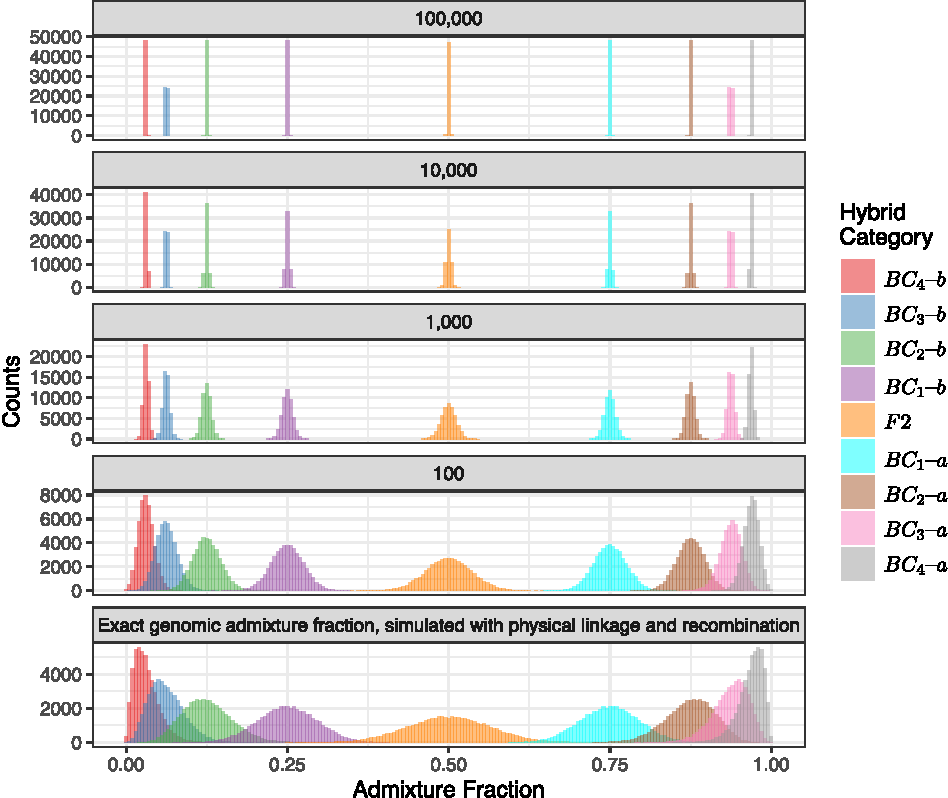
\includegraphics[width=\columnwidth]{figures/link-and-nolink-sims-crop.pdf}
\caption[\adfcap]{\adfcap}
\label{fig:ad-fract-sims}
\end{figure}
%%%%%%%%%%
If markers are assumed to be unlinked, then the variance around the $Q$ estimates of different 
hybrid categories continually declines as more markers are added, from 100, to 100,000, which 
makes it appear that different hybrid categories become increasingly well-resolved.  For example, 
looking at the distributions for 100,000 unlinked markers one would think that it would be easy to 
distinguish between the $BC_1$ through $BC_4$ categories on the basis of the admixture fractions.
This is, however, not the case.  The bottom panel of Fig.\ref{fig:ad-fract-sims} shows the distribution
of the true admixture fraction (calculated as the total length of genome from each of the two
different species) of each individual when simulated with physical linkage using \gscramble{}.
When physical linkage is not ignored, it is quite clear that there is considerable overlap in the
admixture fractions between the $BC_1$ and $BC_2$ categories, and that $BC_2$, $BC_3$, and 
$BC_4$ all have admixture fraction distributions that overlap greatly.  This shows that,
in real life, when physical linkage cannot be ignored, it may be quite difficult to distinguish
between different backcross categories on the basis of their admixture fractions.



\subsection*{Examples}

\subsubsection*{No RISPI when using \gscramble{}}

As expected, there was no RISPI apparent in the ADMIXTURE-estimated
ancestry proportions  when simulating individuals
using \gscramble{} (Fig.~\ref{fig:norispi}).  On average, the estimated $Q$ values
were around 0.5, which is expected when the samples are drawn from the same
population.
%%%
\begin{figure}
\newcommand{\gssimcap}{\footnotesize ADMIXTURE estimates of ancestry
fractions, $Q$, for individuals simulated from samples from the same population,
simulated using \gscramble{}.  There is a considerable variation in the estimates,
but the central tendency of them all is around 0.5, as would be expected in this case
within which there is not genetic basis for distinguishing individuals from the different
samples.  Contrast this to the corresponding panel ($L=1,000, N=50$) in Fig.~\ref{fig:bias-sims}(b),
in which the RISPI is readily apparent.}
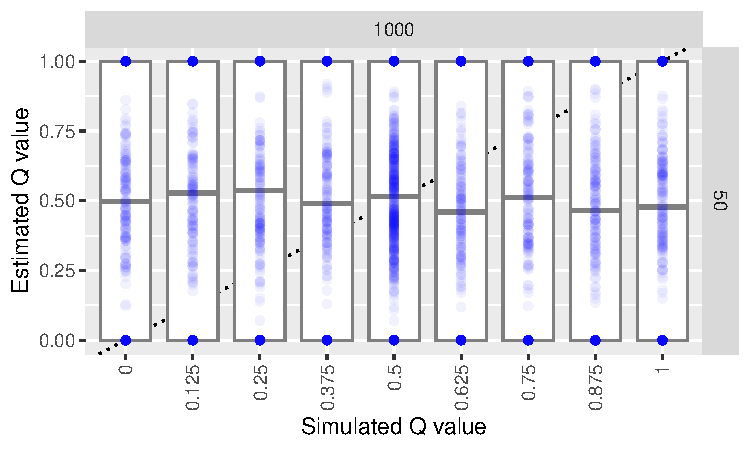
\includegraphics[width=\columnwidth]{figures/gscram_supervised_Qs.pdf}
\caption[\gssimcap]{\gssimcap}
\label{fig:norispi}
\end{figure}
%%%

\subsubsection*{Rainbow/cutthroat trout hybrids in California}

The barplots in Fig.~\ref{fig:newhyb-sims-barplot} show the distribution of posterior
probabilities of the different hybrid categories. 

%%%%%%%%%%
\begin{figure}
\newcommand{\nhbpcap}{\footnotesize Posterior probabilities for simulated
individuals of different trout hybrid categories.  Each pair of plots shows the results
for individuals of the true hybrid category listed atop the pair.  (See Table~\protect\ref{tab:newhybcats} for meaning of the names.)  The top panel of each pair
shows results for fish simulated with the 30 markers used by \protect\citet{rizza2023limited}, and the bottom panel shows results for fish simulated with the original 30 markers,
plus an additional  35 (65 total), some of which are linked
on the same chromosome. Each individual appears as a thin vertical line, posterior probabilities of
each inferred hybrid category are indicated by extent of different colors on those lines.  Individuals
are sorted according to maximum {\em a posteriori} hybrid category, and, within that by the
maximum posterior probability. }
{\centering
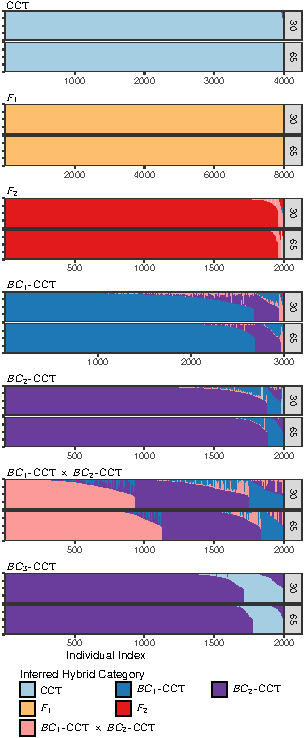
\includegraphics[width=0.98\columnwidth]{figures/newhybs-texed-crop.pdf}
}
\caption[\nhbpcap]{\nhbpcap}
\label{fig:newhyb-sims-barplot}
\end{figure}
%%%%%%%%%%
These are similar to ADMIXTURE barplots;
however, rather than plotting the ancestry fraction, the different colors are showing the
posterior probabilities of different hybrid categories.  Each individual is represented by a thin
vertical line, and the individuals have been arranged from left to right and the colors have been
arranged from top to bottom throughout different sections of the plot to make it easy to see
the patterns.  The {\em maximum-a-posteriori} (MAP) hybrid category for any individual is represented
by the color that is on the bottom of the bar, so it is easy to see the shifts where the MAP hybrid
category changes from one to another.  It is apparent over all individuals simulated to be
either CCT, $F_1$, $F_2$, $BC_1$--CCT, or $BC_2$--CCT, that the MAP estimate of their
hybrid categories were correct for largely the same number of individuals whether 30 or 65 markers
were used. By contrast, for the individuals simulated to be of the complex hybrid category
$BC_1$--CCT~$\times$~$BC_2$--CCT, the MAP estimate from 65 markers was correct more often 
than from 
30 markers.  However, it is also apparent that using 65 markers, some of which are physically
linked, in the software {\em NewHybrids}---which assumes that all markers are unlinked---yields 
estimates of uncertainty that are inaccurate.  Tellingly, when the estimates using 65 markers are 
incorrect (for example, when $BC_1$--CCT individuals have a maximum posterior of being in the 
$BC_2$--CCT category,
or when individuals that are truly of the $BC_1$--CCT~$\times$~$BC_2$--CCT category have a
maximum posterior of being from the $BC_2$--CCT category), many of those incorrect posteriors
are quite high ($>0.90$).  In fact, using 65 markers yields more incorrect {\em and high} posteriors 
than does using the 30 unlinked markers. So, as expected, ignoring physical linkage the way
{\sc NewHybrids} does can yield a poor estimate of the certainty around different inferences.

\subsubsection*{Invasive wild pigs in Missouri}

SNP filtering resulted in 14,233 loci that were used for subsequent analysis.
Using the 160 empirical samples, ADMIXTURE results supported the identification of
$K=3$ genetic clusters grouped individuals from each of the core populations into 3 clusters
while the 40 individuals from the contact regions were highly admixed. The
$F_\mathrm{ST}$ divergence from ADMIXTURE was:
$F_\mathrm{ST} = 0.24$ for Pop1-Pop2,
$F_\mathrm{ST} = 0.14$ for Pop1-Pop3 and
$F_\mathrm{ST} = 0.13$ for Pop2-Pop3.

The simulated hybrid classes produce
the expected range of admixture with $F_1$ and $F_2$ individuals having mean $Q=0.5$, with $F_2$ individuals having
more variation (Figure~\ref{fig:pig-sim-qs}A).
Backcrossed individuals have higher ancestry associated with the backcrossed population with mean $Q$
approximately $0.75$ ($\BC_1$) and $0.87$ ($\BC_2$) (Figure~\ref{fig:pig-sim-qs}A). Notably, the simulated
$F_1$ hybrids have the most variation in the distribution of the $Q$ values associated with each of the genetic clusters.
When the estimated Q values for the $F_1$ hybrids are separated by the population combinations,
$F_1$ hybrids for Pop1-Pop2 have the least variation around $q=0.5$ (standard deviation
= 0.008), while Pop1-Pop3 and Pop2-Pop3
have higher variation (standard deviation = 0.011-0.016) (Figure~\ref{fig:pig-sim-qs}B). Also, all $Q$
distributions for $F_1$ hybrids, regardless of population combination, center around
$0.50$ except for the two distributions
of Pop3, which have a mean of $Q=0.49$ (Figure~\ref{fig:pig-sim-qs}B).
The differences among these
distributions of $Q$ values for the simulated data reflect the genetic differences observed
in the empirical data, specifically, that genetic differentiation is highest between Pop1 and Pop2 and that
Pop14 is the most admixed population with ancestry contributions from both Pop1 and Pop2.


%%%
\begin{figure}
\newcommand{\pigsimsqscap}{\footnotesize (A) The density of the estimated Q values from ADMIXTURE for
the simulated runs are
grouped across all population-combinations for each hybrid class and colored by the $K$ genetic cluster
(e.g., the Pop1 density plot for the $\BC_1$ plots the Pop1 genetic cluster for both
the Pop1-Pop2 and Pop1-Pop3 combinations). The density plots across the $K$
genetic clusters are mostly similar with the most variation among the genetic clusters evident in
the $F_1$ plot. (B) Plotting the density of the estimated Q values from ADMIXTURE for the $F_1$ hybrids,
separated by the population combinations, reveals the least variance in estimated Q values for
Pop1-Pop2 compared to Pop1-Pop3 and Pop2-Pop3. Note that these population combinations group the
reciprocal population combination in each plot (e.g., "Pop1\_Pop2" has simulations
from both Pop1-Pop2 and Pop2-Pop1).}
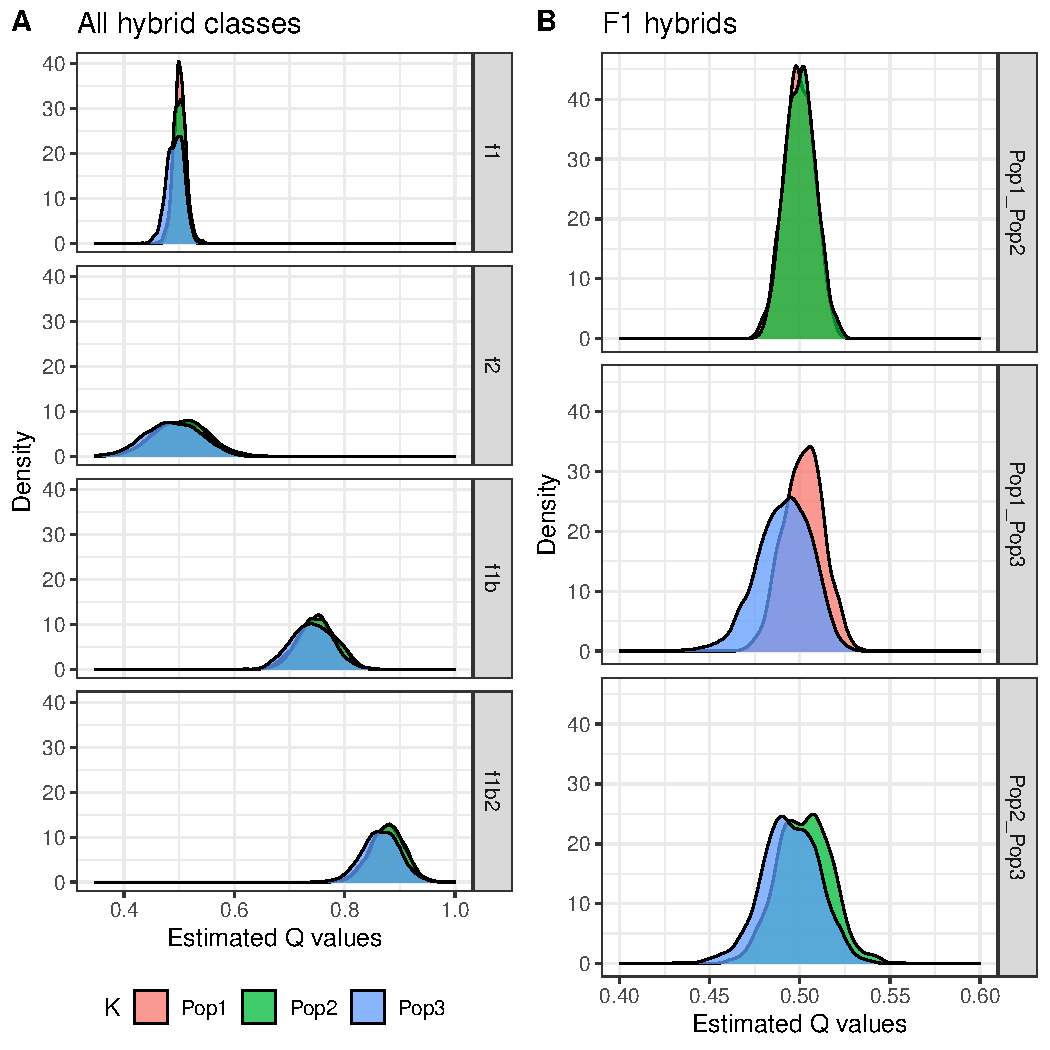
\includegraphics[width=\columnwidth]{figures/simulation-density-multipanel.pdf}
\caption[\pigsimsqscap]{\pigsimsqscap}
\label{fig:pig-sim-qs}
\end{figure}
%%%

\section*{Discussion}

Somewhere here I want to mention that the Anderson et al. (2008) approach for simulating
mixtures of genotypes to assess how well one can estimate mixture proportions---the fraction
of individuals from each of a set of baseline or reference populations---allows the user to
simulate, if desired, more genotypes than occur in the reference samples.  This is because
a trick is done in the inference stage to remove the correlation between the simulated individual
and the reference sample, relative to the true population, by removing the simulated individual's
genotypes from its own reference population when calculating the likelihood that its genotype
originated from each of the reference populations.  To do the same when doing simulations for
assessing power using ADMIXTURE or STRUCTURE would require hacking the underlying code
of those programs, which is not desirable.  So, for these cases we have used the sampling
without replacement approach.

Also, we need to discuss the fact that, because each time a gamete is segregated in the
pedigree, its complement is also segregated, this is an example of antithetical variate sampling
in Monte Carlo.  

\section*{Acknowledgements}
Research was supported in part by the USDA-APHIS-National Feral Swine Damage
Management Program. We are grateful for the numerous Wildlife Services and Missouri
Department of Conservation employees that contributed to genetic sampling of wild pigs
within southeastern Missouri. We thank Yniv Palti for providing flanking sequences and the linkage map for 57K markers for making a recombination map for the cutthroat/rainbow trout example. Writing of this paper was facilitated by the Mobile High Altitude Venue for Ecological Analysis,
Genetics and Statistics, through which ECA, MGD, and TJS were scientists-in-residence on location in
Cheyenne, WY for 3 days in October 2023. This is contribution number mHAVEAGAS-003.
This work utilized the Alpine high performance computing resource at the University of Colorado Boulder.
Alpine is jointly funded by the University of Colorado Boulder, the University of Colorado Anschutz, Colorado State University,
and the National Science Foundation (award 2201538).
